%%%
% Plantilla de Memoria
% Modificación de una plantilla de Latex de Nicolas Diaz para adaptarla 
% al castellano y a las necesidades de escribir informática y matemáticas.
%
% Editada por: Mario Román
%
% License:
% CC BY-NC-SA 3.0 (http://creativecommons.org/licenses/by-nc-sa/3.0/)
%%%

%%%%%%%%%%%%%%%%%%%%%%%%%%%%%%%%%%%%%%%%%
% Thin Sectioned Essay
% LaTeX Template
% Version 1.0 (3/8/13)
%
% This template has been downloaded from:
% http://www.LaTeXTemplates.com
%
% Original Author:
% Nicolas Diaz (nsdiaz@uc.cl) with extensive modifications by:
% Vel (vel@latextemplates.com)
%
% License:
% CC BY-NC-SA 3.0 (http://creativecommons.org/licenses/by-nc-sa/3.0/)
%
%%%%%%%%%%%%%%%%%%%%%%%%%%%%%%%%%%%%%%%%%

%----------------------------------------------------------------------------------------
%	PAQUETES Y CONFIGURACIÓN DEL DOCUMENTO
%----------------------------------------------------------------------------------------
%%% Configuración del papel.
% microtype: Tipografía.
% mathpazo: Usa la fuente Palatino.
\documentclass[a4paper, 11pt]{article}
\usepackage[protrusion=true,expansion=true]{microtype}
\usepackage{mathpazo}


% Indentación de párrafos para Palatino
\setlength{\parindent}{0pt}
  \parskip=8pt
\linespread{1.05} % Change line spacing here, Palatino benefits from a slight increase by default


%%% Castellano.
% noquoting: Permite uso de comillas no españolas.
% lcroman: Permite la enumeración con numerales romanos en minúscula.
% fontenc: Usa la fuente completa para que pueda copiarse correctamente del pdf.
\usepackage[spanish,es-noquoting,es-lcroman]{babel}
\usepackage[utf8]{inputenc}
\usepackage[T1]{fontenc}
\selectlanguage{spanish}


%%% Gráficos
\usepackage{graphicx} % Required for including pictures
\usepackage{wrapfig} % Allows in-line images
\usepackage[usenames,dvipsnames]{color} % Coloring code

%%% Matemáticas
\usepackage{amsmath}


%%% Bibliografía
\makeatletter
\renewcommand\@biblabel[1]{\textbf{#1.}} % Change the square brackets for each bibliography item from '[1]' to '1.'
\renewcommand{\@listI}{\itemsep=0pt} % Reduce the space between items in the itemize and enumerate environments and the bibliography
\usepackage{hyperref}
\hypersetup{
	colorlinks   = true,    % Colours links instead of ugly boxes
	urlcolor     = red,    % Colour for external hyperlinks
	linkcolor    = red,    % Colour of internal links
	citecolor    = blue      % Colour of citations
}

%%% CÓDIGO

\usepackage{listings}   
\usepackage{xcolor}
\lstdefinestyle{customc}{	
	backgroundcolor=\color{white},    % choose the background color; you must add \usepackage{color} or \usepackage{xcolor}; should come as last argument
	basicstyle=\footnotesize\ttfamily,% the size of the fonts that are used for the code
	breakatwhitespace=false,          % sets if automatic breaks should only happen at whitespace
	breaklines=true,                  % sets automatic line breaking
	captionpos=b,                     % sets the caption-position to bottom
    commentstyle=\itshape\color{purple!40!black},     % comment style
	deletekeywords={...},             % if you want to delete keywords from the given language
	escapeinside={\%*}{*)},           % if you want to add LaTeX within your code
	extendedchars=true,               % lets you use non-ASCII characters; for 8-bits encodings only, does not work with UTF-8
	frame=single,	                  % adds a frame around the code
	keepspaces=true,                  % keeps spaces in text, useful for keeping indentation of code (possibly needs columns=flexible)
	keywordstyle=\bfseries\color{green!40!black},       % keyword style
	language=C,                       % the language of the code
	morekeywords={*,...},             % if you want to add more keywords to the set
	numbers=left,                     % where to put the line-numbers; possible values are (none, left, right)
	numbersep=5pt,                    % how far the line-numbers are from the code
	numberstyle=\tiny\color{gray},    % the style that is used for the line-numbers
	rulecolor=\color{black},          % if not set, the frame-color may be changed on line-breaks within not-black text (e.g. comments (green here))
	showspaces=false,                 % show spaces everywhere adding particular underscores; it overrides 'showstringspaces'
	showstringspaces=false,           % underline spaces within strings only
	showtabs=false,                   % show tabs within strings adding particular underscores
	stepnumber=2,                     % the step between two line-numbers. If it's 1, each line will be numbered
    stringstyle=\color{orange},       % string literal style
	tabsize=2,	                      % sets default tabsize to 2 spaces
	title=\lstname,                   % show the filename of files included with \lstinputlisting; also try caption instead of title
	identifierstyle=\color{blue}
}

\lstdefinestyle{customasm}{
	belowcaptionskip=1\baselineskip,
	frame=L,
	xleftmargin=\parindent,
	language=[x86masm]Assembler,
	basicstyle=\footnotesize\ttfamily,
	commentstyle=\itshape\color{purple!40!black},
}

\DeclareFixedFont{\ttb}{T1}{txtt}{bx}{n}{8} % for bold
\DeclareFixedFont{\ttm}{T1}{txtt}{m}{n}{8}  % for normal


\lstdefinestyle{customPY}{
	language=Python,
	basicstyle=\ttm,
	otherkeywords={self},             % Add keywords here
	keywordstyle=\ttb\color{blue},
	emph={MyClass,__init__},          % Custom highlighting
	emphstyle=\ttb\color{red},    % Custom highlighting style
	stringstyle=\color{orange},
	frame=tb,                         % Any extra options here
	showstringspaces=false       
}

\lstset{escapechar=@,style=customc}


%% cosas 

\usepackage[margin=1in]{geometry}

\usepackage{times}


%----------------------------------------------------------------------------------------
%	TÍTULO
%----------------------------------------------------------------------------------------
% Configuraciones para el título.
% El título no debe editarse aquí.
\renewcommand{\maketitle}{
  \begin{flushright} % Right align
  
  {\LARGE\@title} % Increase the font size of the title
  
  \vspace{50pt} % Some vertical space between the title and author name
  
  {\large\@author} % Author name
  \\\@date % Date
  \vspace{40pt} % Some vertical space between the author block and abstract
  \end{flushright}
}

%% Título
\title{\textbf{Construyendo sobre Prelude}\\ % Title
					una introducción a Emacs.} % Subtitle

\author{\textsc{Francisco Navarro Morales} % Author
\\{\textit{GRG121}}} % Institution

\date{\today} % Date





%----------------------------------------------------------------------------------------
%	DOCUMENTO
%----------------------------------------------------------------------------------------

\begin{document}
	
	
	\begin{titlepage}
		\begin{center}
			\vspace*{2cm}
			
			{\Huge \textbf{¿Y qué si P = NP?}}
			
			 ALGORITMICA 
			
			
			\vspace{0.5cm}
			
			
		    \centering 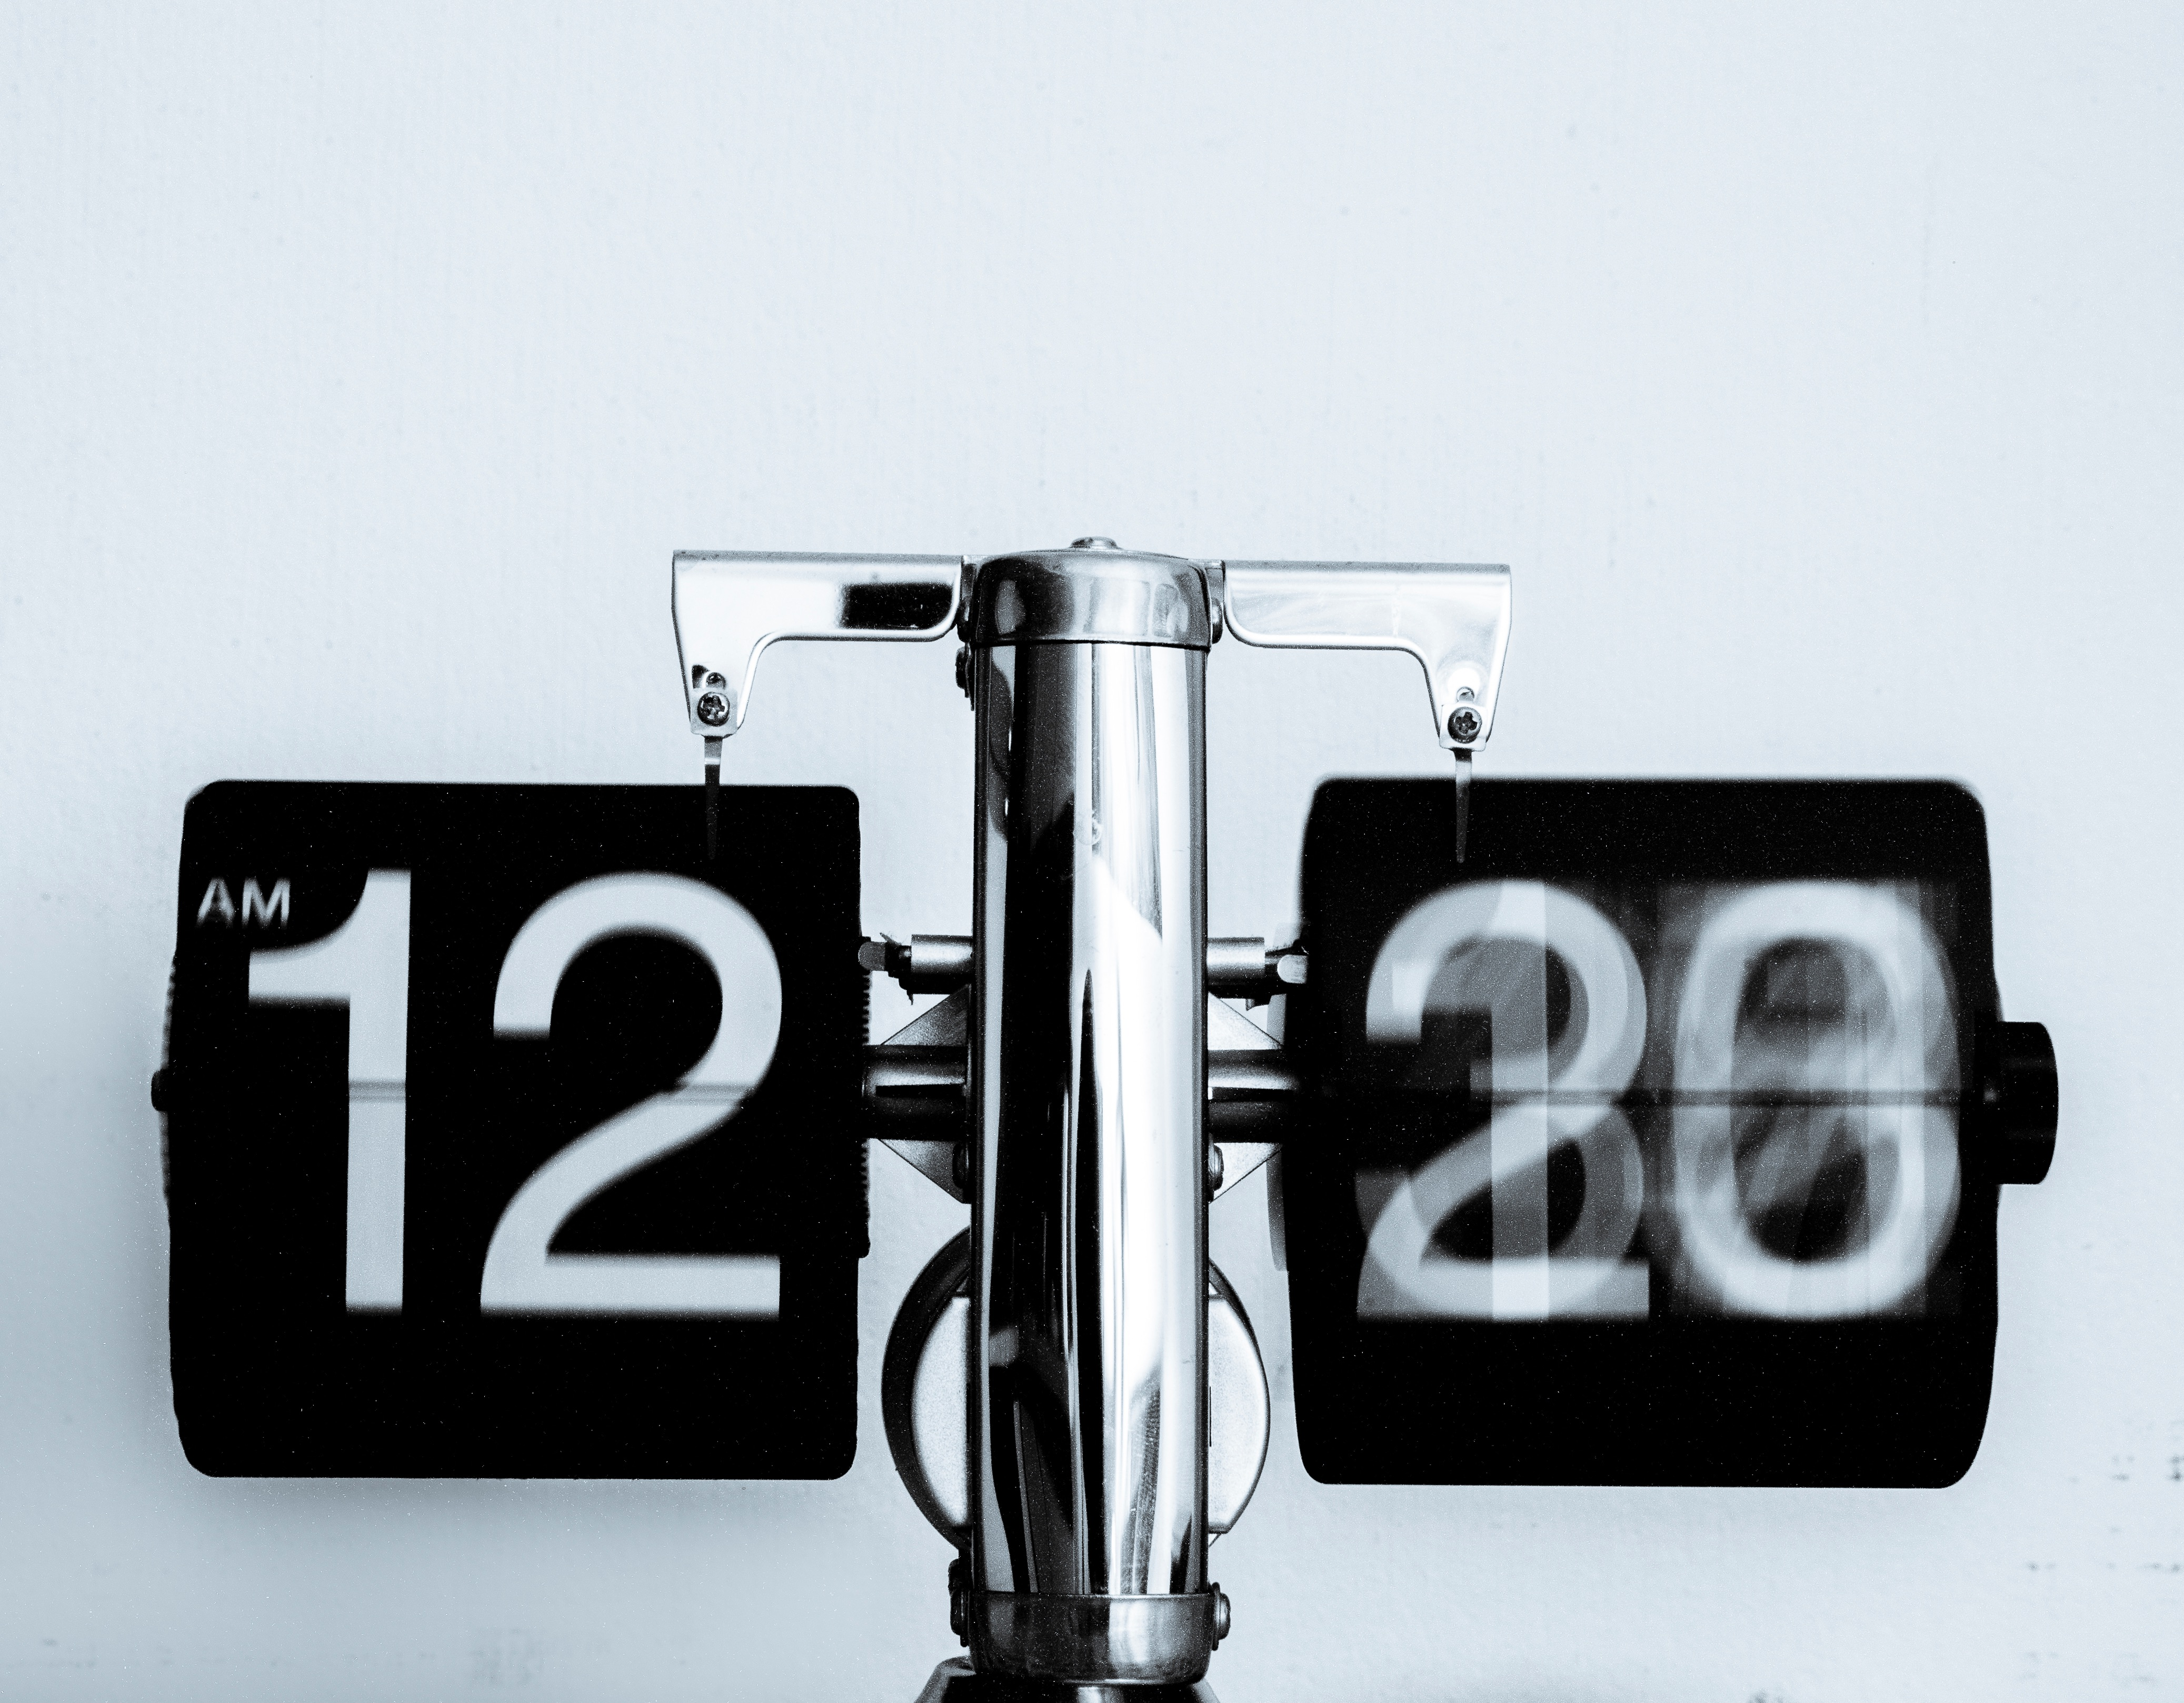
\includegraphics[width=0.7\textwidth]{cover.jpg}
		    
		    
		    {\footnotesize Photo Loic Djim on unsplash.com}
			
			\vspace{2cm}
			
			\textbf{Francisco Navarro Morales - GRG121 }
			
			\vfill
			
			Segundo curso del Grado de Ingeniería Informática\\
			Universidad de Granada\\
			curso 2016-2017\\
			
		\end{center}
	\end{titlepage}


%\maketitle % Print the title section

%% Resumen (Descomentar para usarlo)
\renewcommand{\abstractname}{Resumen} % Uncomment to change the name of the abstract to something else
%\begin{abstract}
% Resumen aquí
%\end{abstract}

%% Palabras clave
%\hspace*{3,6mm}\textit{Keywords:} lorem , ipsum , dolor , sit amet , lectus % Keywords
%\vspace{30pt} % Some vertical space between the abstract and first section


%% Índice
%%{\parskip=2pt
%%  \tableofcontents
%%}

%%% Inicio del documento

\pagebreak


Llamamos problemas P a aquellos para los que existe un algoritmo eficiente (tiempos de ejecución como funciones polinomiales) que puede ejecutarse en una maquina de Turing determinista, y NP a aquellos problemas para los que la única manera de obtener una respuesta en tiempo eficiente es a través de una etapa aleatoria en la que se establece una solución al azar y se comprueba en tiempo eficiente si esta es correcta. Sin embargo, debido a ese factor aleatorio, los tiempos deseados pueden no darse; para asegurar la ejecución en tiempo eficiente (orden polinómico) necesitaríamos una máquina de Turing no determinista (concepto ficticio), que sería algo así como una máquina capaz de "duplicarse" y realizar tantas operaciones en paralelo como quisiera. 

Ahora bien, \textbf{ ¿es P = NP?}

Podemos afirmar que $ P \subseteq NP $ puesto que, cualquier problema para el que exista un algoritmo con eficiencia de orden polinómico podría ser resuelto por los métodos propios de algoritmos NP; esto es, una maquina de Turing no determinista podría ejecutar cualquier problema P simplemente no clonándose ninguna vez. Ahora bien, si $NP \subseteq P $ y, por tanto $ P = NP $, entonces significaría que cualquier algoritmo de la clase NP podría realizarse en un orden de tiempo polinómico con una máquina de Turing determinista y, por tanto, las implicaciones serían cuantiosas.

Y es que, si por ejemplo, necesitáramos encontrar la clave para desencriptar un fichero, una máquina de Turing no determinista podría comprobar todas las claves posibles y determinar cual es la correcta en el mismo tiempo en que una máquina determinista comprobaría si una clave es correcta; sin embargo, dado que las máquinas no deterministas son sólo elementos teóricos, conseguir desencriptar un archivo en tiempo eficiente es imposible. Sin embargo, si $ P = NP $, entonces existe un algoritmo tal que una máquina determinista (a las cuales sí tenemos acceso) podría realizar la labor que comentábamos propia de una no determinista en el mismo orden de tiempo, proporcionándonos la posibilidad de desencriptar cualquier archivo (que haya sido encriptado teniendo en cuenta las propiedades de los problemas NP) en un tiempo muy breve.

Esto supone aún más, si supiéramos que $P = NP$ significaría que es sólo cuestión de tiempo ir encontrando algoritmos polinómicos para problemas de la clase NP y, al encontrarlos, podríamos conseguir respuestas para las que esperamos durante meses o años, en cuestión de horas, minutos o segundos; es decir, podríamos obtener una respuesta para la que un supercomputador ha estado trabajando durante un año en menos de una hora sin necesidad de un ordenador especialmente potente, y obtener respuestas que nos sería imposible obtener a día de hoy. Imagina una pregunta para la cual una computadora podría ofrecer una respuesta dentro de 1000 años, la única manera que tendríamos a día de hoy de saber esa respuesta antes de morir sería (aunque es casi tan improbable como vivir 1000 años) viajar en el tiempo para ver la respuesta que dará el ordenador dentro de 1000 años, y luego volver para poder compartirla. Sin embargo, si $P = NP$, entonces no necesitaríamos ese hipotético viaje en el tiempo, podríamos adelantar la respuesta a nuestro tiempo.

Además, esto supondría sin lugar a dudas una nueva revolución tecnológica puesto que permitiría el avance de numerosos estudios en muy poco tiempo y el desarrollo mucho más eficiente de nuevas tecnologías. No obstante, aunque aún es una cuestión abierta, los indicios actuales apuntan a que $P != NP$, que es la principal hipótesis de los que intentan encontrar una demostración matemática al respecto, ya que parece imposible que fuera real que $P = NP$. En caso de que la mayoría tuviera razón y $P != NP$, lo único que ganaríamos sería la certeza de que nuestros sistemas actuales de encriptación son seguros, y que es una pérdida de tiempo intentar encontrar soluciones eficientes a los problemas NP, pero esto no supondría ninguna revolución científica ni mucho menos. Es por esto que quizá sería conveniente no descartar del todo la posibilidad de que todos los problemas pertenezcan a un mismo grupo hasta que se demuestre lo contrario, pues si algún día se llegara a demostrar que esta hipótesis es correcta, se produciría un avance tecnológico que afectaría a todo el mundo. 




\end{document}